\documentclass{article}

\usepackage{tikz}
%\usepackage{rotating}
 

\begin{document}
%\begin{turn}{90}
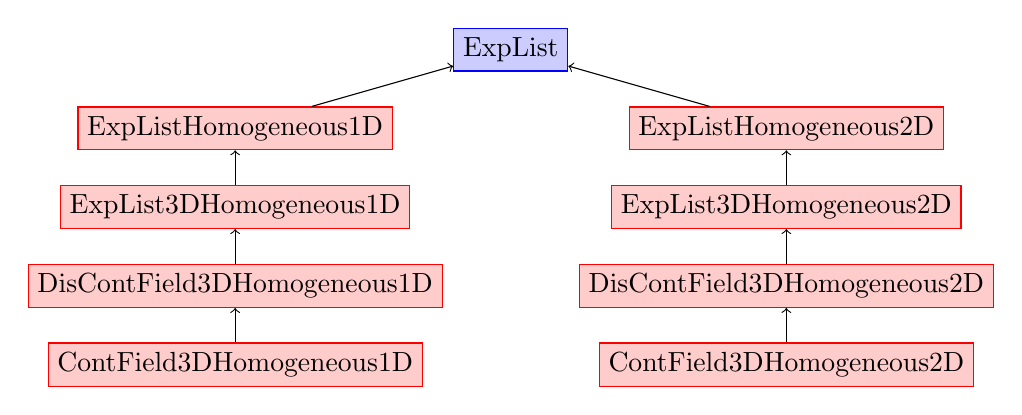
\begin{tikzpicture}[outline/.style={draw=#1,fill=#1!20}]

%NODES

% level (1) 
\node [outline=blue] (ExpList)                                   at (4.5,0)          {ExpList};
% level (2) y = -2
\node [outline=red] (ExpListHomogeneous1D)                              at (1,-1)        {ExpListHomogeneous1D};
\node [outline=red] (ExpListHomogeneous2D)                              at (8,-1)        {ExpListHomogeneous2D};
% level (3) 
\node [outline=red] (ExpList3DHomogeneous1D)                    at (1,-2)         {ExpList3DHomogeneous1D};
\node [outline=red] (ExpList3DHomogeneous2D)                    at (8,-2)         {ExpList3DHomogeneous2D};
% level (3) 
\node [outline=red] (DisContField3DHomogeneous1D)                    at (1,-3)        {DisContField3DHomogeneous1D};
\node [outline=red] (DisContField3DHomogeneous2D)                    at (8,-3)         {DisContField3DHomogeneous2D};
% level (4) 
\node [outline=red] (ContField3DHomogeneous1D)                    at (1,-4)        {ContField3DHomogeneous1D};
\node [outline=red] (ContField3DHomogeneous2D)                    at (8,-4)         {ContField3DHomogeneous2D};

%CONNECTIONS

\path[<-]  (ExpList)      edge (ExpListHomogeneous1D)
                 (ExpList)      edge (ExpListHomogeneous2D)
                
                 (ExpListHomogeneous1D) edge (ExpList3DHomogeneous1D)
                 (ExpListHomogeneous2D) edge (ExpList3DHomogeneous2D)
                 
                 (ExpList3DHomogeneous1D)  edge (DisContField3DHomogeneous1D)
                 (ExpList3DHomogeneous2D)  edge (DisContField3DHomogeneous2D)
                 
                 (DisContField3DHomogeneous1D)  edge (ContField3DHomogeneous1D)
                 (DisContField3DHomogeneous2D)  edge (ContField3DHomogeneous2D);
\end{tikzpicture}
%\end{turn}

\end{document}